\documentclass[english,hebrew]{article}
\usepackage[HE8,T1]{fontenc}
\usepackage[utf8]{inputenc}
\setcounter{secnumdepth}{-2}
\setlength{\parindent}{0bp}
\usepackage{amsmath}
\usepackage{amsthm}
\usepackage{amssymb}
\usepackage{graphicx}

\makeatletter
\newlength{\lyxlabelwidth}      % auxiliary length 
\theoremstyle{remark}
\newtheorem*{rem*}{\protect\remarkname}

\@ifundefined{date}{}{\date{}}
\usepackage{graphicx}
\usepackage{geometry}
\newcommand{\limi}{\underset{n\rightarrow\infty}{\lim}}
\newcommand{\limxz}{\underset{x\rightarrow x_{0}}{\lim}}
\newcommand{\limfxz}{\underset{x\rightarrow x_{0}}{\lim}f(x)}
\newcommand{\limfxm}{\underset{x\rightarrow x_{0}^{-}}{\lim}f(x)}
\newcommand{\limfxp}{\underset{x\rightarrow x_{0}^{+}}{\lim}f(x)}
\newcommand{\limxm}{\underset{x\rightarrow x_{0}^{-}}{\lim}}
\newcommand{\limxp}{\underset{x\rightarrow x_{0}^{+}}{\lim}}
\newcommand{\sqrm}{M_{m\times m}(\mathbb{F})}
\newcommand{\seqa}{(a_{n})_{n=1}^{\infty}}
\newcommand{\seqx}{(x_{n})_{n=1}^{\infty}}
\newcommand{\funcdr}{f:D\rightarrow\mathbb{R}}
\newcommand{\der}{\limxz\frac{f(x)-f(x_{0})}{x-x_{0}}}
\usepackage[all]{pdfprivacy}

\makeatother

\usepackage{babel}
\addto\captionsenglish{\renewcommand{\remarkname}{Remark}}
\addto\captionshebrew{\renewcommand{\remarkname}{הערה}}
\providecommand{\remarkname}{הערה}

\begin{document}
\newgeometry{top=1cm, bottom=2cm, left=1cm, right=1cm}
\title{רציפות במ\textquotedblright ש וליפשיציות}
\author{נעם לב}

\maketitle
\textbf{הגדרה - רציפות במידה שווה}

תהי \L{$D\subseteq\mathbb{R}$} ותהי \L{$f:D\to\mathbb{R}$} פונקציה
נתונה. נאמר ש-\L{$f$} \textbf{רציפה במידה שווה ב-}\L{$D$} אם"ם

\L{%
\[
\forall\varepsilon>0\quad\exists\delta>0\quad\forall x_{1},x_{2}\in D\qquad|x_{2}-x_{1}|<\delta\Rightarrow|f(x_{2})-f(x_{1})|<\varepsilon
\]
}%

\textbf{דוגמה:}

הפונקציה \L{$f:\mathbb{R}\to\mathbb{R}$} המוגדרת על ידי \L{$f(x)=\sin(x)$}
רציפה במידה שווה ב-\L{$\mathbb{R}$}.

בהינתן \L{$\varepsilon>0$}, נבחר \L{$\delta=\varepsilon$} ואז לכל
\L{$x_{1},x_{2}\in\mathbb{R}$} כך ש- \L{$|x_{2}-x_{1}|<\delta=\varepsilon$}
מתקיים:

\L{%
\begin{align*}
|f(x_{2})-f(x_{1})| & =|\sin(x_{2})-\sin(x_{1})|=\left|2\sin\left(\frac{x_{2}-x_{1}}{2}\right)\cos\left(\frac{x_{2}+x_{1}}{2}\right)\right|=2\left|\sin\left(\frac{x_{2}-x_{1}}{2}\right)\right|\left|\cos\left(\frac{x_{2}+x_{1}}{2}\right)\right|\\
 & \leqslant2\left|\sin\left(\frac{x_{2}-x_{1}}{2}\right)\right|\cdot1\leqslant2\left|\frac{x_{2}-x_{1}}{2}\right|=|x_{2}-x_{1}|<\delta=\varepsilon
\end{align*}
}%

\textbf{הגדרה - פונקציה ליפשיצית}

נאמר שפונקציה \L{$f:D\to\mathbb{R}$} היא \textbf{פונקציה ליפשיצית
על \L{$D$}} )או מקיימת את תנאי ליפשיץ ב-\L{$D$}( אם קיים קבוע \L{$K\geq0$}
)הנקרא קבוע ליפשיץ( כך שלכל שתי נקודות \L{$x_{1},x_{2}\in D$} מתקיים:

\L{%
\[
|f(x_{2})-f(x_{1})|\leq K\cdot|x_{2}-x_{1}|
\]
}%

במילים אחרות, ליפשיציות מתארת קצב שינוי פונ' שהוא חסום.

בדוגמה ראינו שהפונקציה \L{$\sin(x)$} היא \L{$1$}-ליפשיצית ב-\L{$\mathbb{R}$}.
\begin{rem*}
לפעמים מגדירים ליפשיציות עם \L{$K>0$} ואז לא צריך להתמודד עם המקרה
\L{$K=0$}.
\end{rem*}
\begin{center}
\L{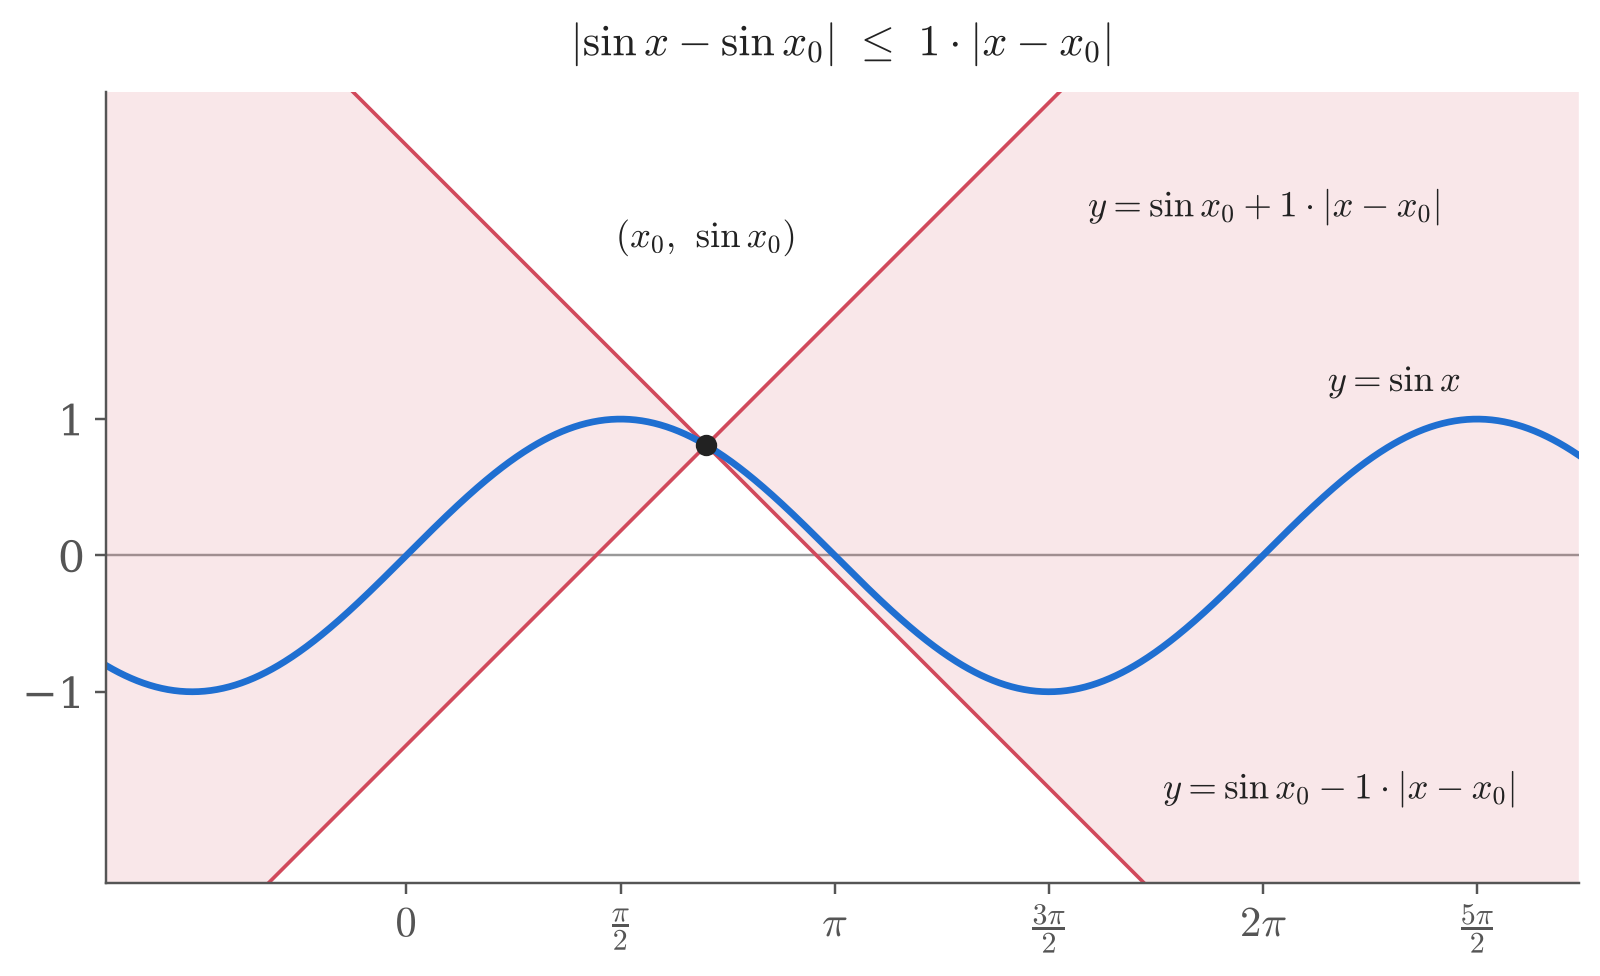
\includegraphics[scale=0.2]{sin-is-1-lipschitz}}
\par\end{center}

\textbf{משפט - ליפשיציות גוררת רציפות במידה שווה}

תהי \L{$f:D\rightarrow\mathbb{R}$} פונ' המקיימת את תנאי ליפשיץ עם
קבוע ליפשיץ \L{$K\ge0$}. 

אזי \L{$f$} היא פונ' רציפה במידה שווה ב-\L{$D$}.\\

וכמובן ראינו שרציפות במידה שווה גוררת רציפות, לכן ליפשיציות גוררת
רציפות.\\

\textbf{הוכחה:}

יהי \L{$\varepsilon>0$}. נרצה למצוא \L{$\delta>0$} מתאים. נפריד
למקרים.

\textbf{מקרה א' )\L{$K=0$}(:} לפי הגדרת ליפשיץ נקבל שלכל שתי נקודות
\L{$x_{1},x_{2}\in D$} מתקיים \L{$|f(x_{1})-f(x_{2})|\leq0$}, מכאן
\L{$|f(x_{1})-f(x_{2})|=0$}, כלומר הפונקציה היא קבועה וברור כי היא
רציפה במידה שווה )נוכל לבחור \L{$\delta$} שרירותי. נבחר \L{$\delta=1$}
ונקבל \L{$|f(x_{1})-f(x_{2})|=0<\varepsilon$}(.\\

\textbf{מקרה ב' )\L{$K>0$}(:} נבחר \L{$\delta=\frac{\varepsilon}{K}$}.

)מכיוון שגם \L{$\varepsilon$} וגם \L{$K$} הם מספרים חיוביים ממש,
מובטח לנו ש- \L{$\delta>0$} כנדרש(.

יהיו \L{$x_{1},x_{2}\in D$} שתי נקודות כלשהן כך ש- \L{$|x_{1}-x_{2}|<\delta$}.

מכיוון שהפונקציה ליפשיצית, מתקיים:

\L{%
\[
|f(x_{1})-f(x_{2})|\leq K\cdot|x_{1}-x_{2}|<K\cdot\delta=K\cdot\left(\frac{\varepsilon}{K}\right)=\varepsilon
\]
}%

כנדרש.

\hfill{}\L{$\square$}

אנו למדים שאם שיפוע הפונקציה חסום אז היא רציפה במ\textquotedblright ש. 

לכן, מבחינה אינטואיטיבית, כאשר שיפוע הפונקציה גדול כרצוננו נחשוד שהפונקציה
אינה רציפה במ\textquotedblright ש. חשוב לציין שזה לא תמיד נכון ועל
כן רציפות במ\textquotedblright ש היא לא אם\textquotedblright ם ליפשיציות...
דוגמה נגדית היא \L{$\sqrt{x}:[0,1]\rightarrow\mathbb{R}$} .
\begin{center}
\L{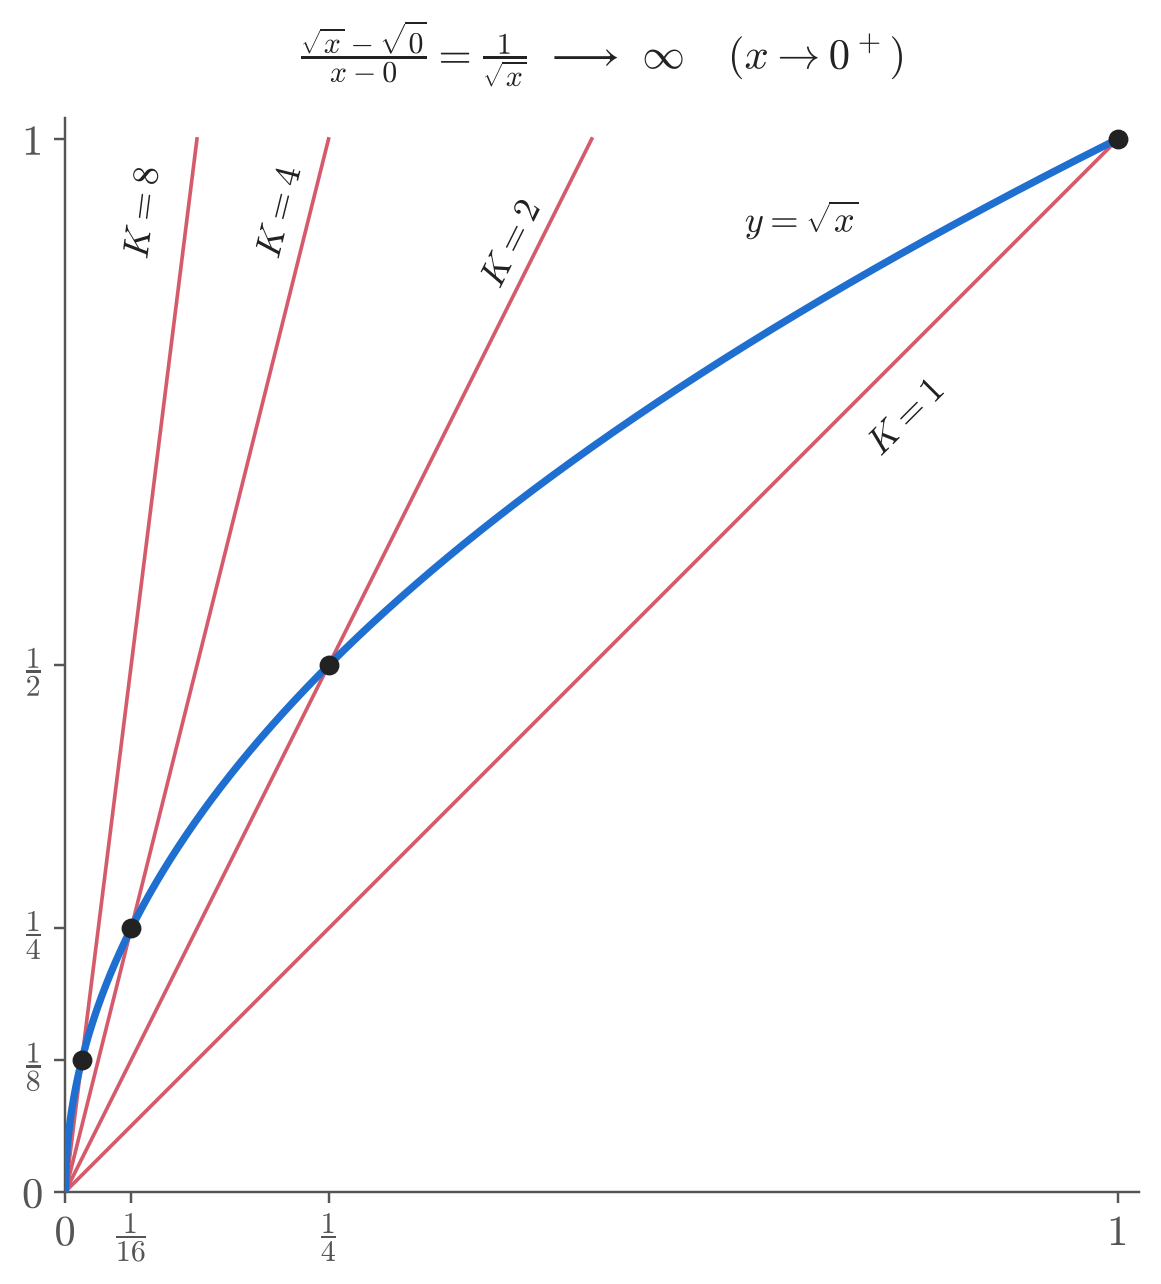
\includegraphics[scale=0.2]{sqrt-is-not-lipschitz}}
\par\end{center}
\end{document}
